% ------- Δ = 0.125 -------
% min :1.14718987543925e-05
% max :22.2868913474062
% q_97.5 : c(`97.5%` = 0.0152186598332864)
% q_95 :c(`95%` = 0.00915432362046129)
% [1] "➤ quantiles extrêmes (> 97.5%) :"
% mc eucl_12_13
% 1:   6  0.1968115
% 2:  91  0.1810575
% 3: 109 13.5030314
% 4: 133  0.1432259
% 5: 157 22.2868913
% ------- Δ = 0.062 -------
%   min :4.35276546353077e-06
% max :67.8923793508904
% q_97.5 : c(`97.5%` = 0.00488494583251508)
% q_95 :c(`95%` = 0.00357287390908308)
% [1] "➤ quantiles extrêmes (> 97.5%) :"
% mc   eucl_12_13
% 1:  6 67.892379351
% 2: 18  0.007600918
% 3: 33  0.005005537
% 4: 67  0.006323381
% 5: 90  0.005215573

\begin{figure}
	\begin{tabularx}{\textwidth}{ccccc}
		\toprule
		statistique sur $\mathcal R_{eucl}$ & \textbf{Individuel} & \textbf{Global} & $\Delta$ & $\lambda$ \\
		\midrule
		\textbf{min}                        & 0.000226            & 0.338           & 0.1      & $\vdots$  \\
		\textbf{max}                        & 36.71               & 2.448           & 0.1      & 60        \\
		\textbf{quantile} $q_{97.5\%}$      & 0.0618              & 1.862           & 0.1      & $\vdots$  \\
		\textbf{quantile} $q_{95\%}$        & 0.0457              & 1.682           & 0.1      & $\vdots$  \\
		\midrule
		\textbf{min}                        & 3.06$\cdot 10^{-6}$ & 0.474           & 0.015    & $\vdots$  \\
		\textbf{max}                        & 83.53               & 2.825           & 0.015    & $\vdots$  \\
		\textbf{quantile} $q_{97.5\%}$      & 0.00322             & 1.909           & 0.015    & 60        \\
		\textbf{quantile} $q_{95\%}$        & 0.00236             & 1.794           & 0.015    & $\vdots$  \\

		\bottomrule
	\end{tabularx}
\end{figure}
% ~ INDIV
% -------Δ = 0.1 - ------
% min:0.000225584627884278
% max:36.7108493938516
% q_97.5:c(`97.5%` = 0.0617630505148869)
% q_95:c(`95%` = 0.0456530021210119)
% -------Δ = 0.015 - ------
%     min:3.06408542204381e-06
% max:83.5292251521978
% q_97.5:c(`97.5%` = 0.00321982597686206)
% q_95:c(`95%` = 0.00236197723089737)
% ~ GLOBAL
% -------Δ = 0.1 - ------
% min:0.338299103983652
% max:2.44757683316762
% q_97.5:c(`97.5%` = 1.86152076412267)
% q_95:c(`95%` = 1.68205548116428)
% -------Δ = 0.015 - ------
% min:0.474057352714499
% max:2.82498526036493
% q_97.5:c(`97.5%` = 1.90935787150105)
% q_95:c(`95%` = 1.79403703076924)

\begin{figure}[H]
	\centering
	\begin{minipage}{\linewidth}
		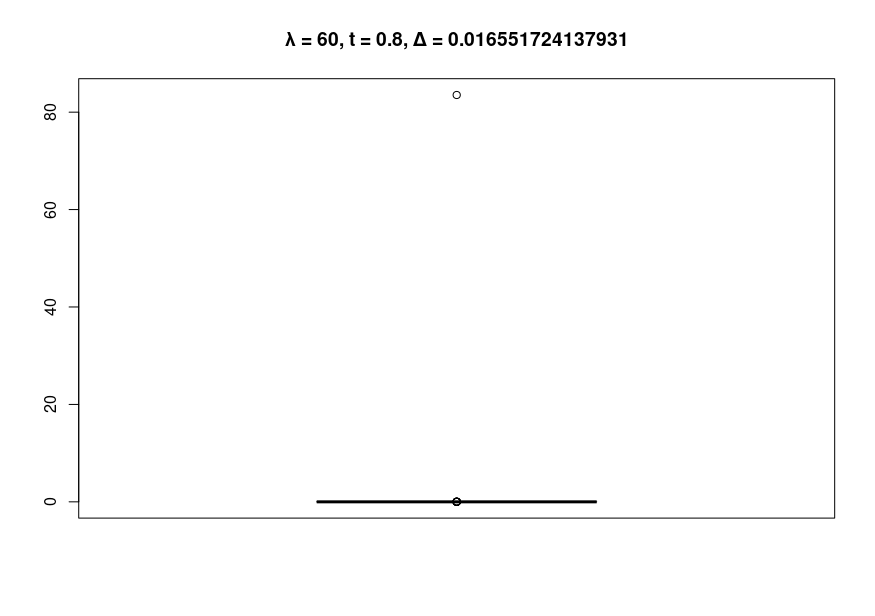
\includegraphics[width=0.47\textwidth]{Images/indiv_vs_glob/qq160.png}
		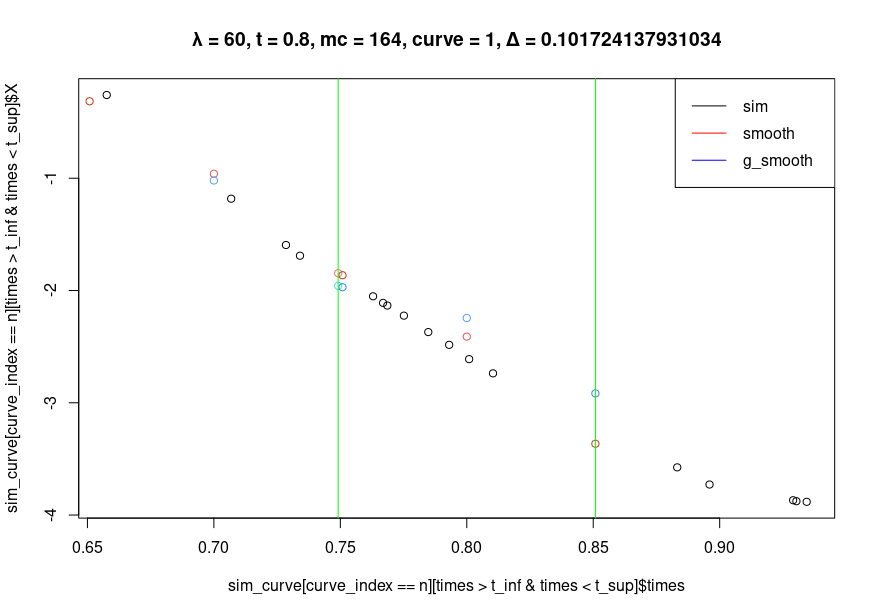
\includegraphics[width=0.47\textwidth]{Images/indiv_vs_glob/lbd60mc164c1.png}
	\end{minipage}

	\begin{minipage}{\linewidth}
		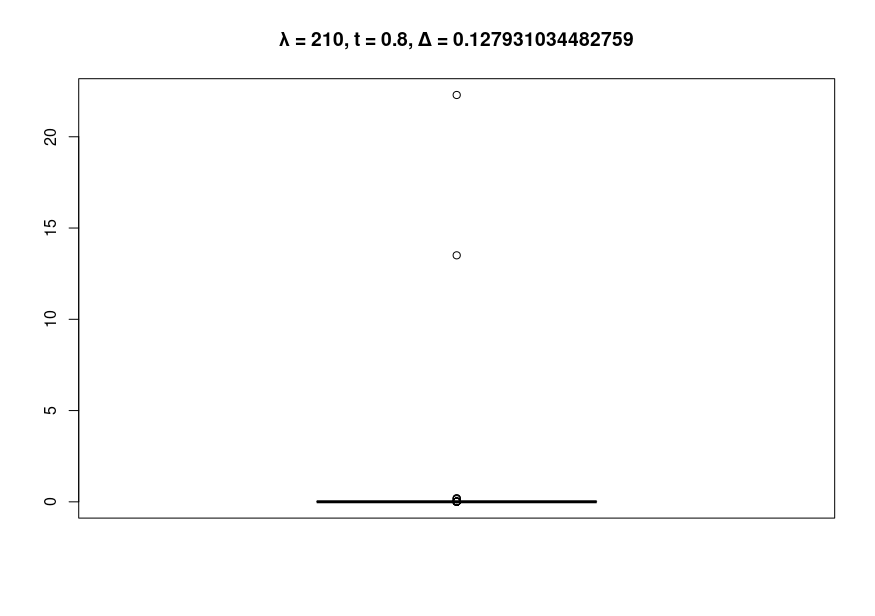
\includegraphics[width=0.47\textwidth]{Images/indiv_vs_glob/qq210.png}
		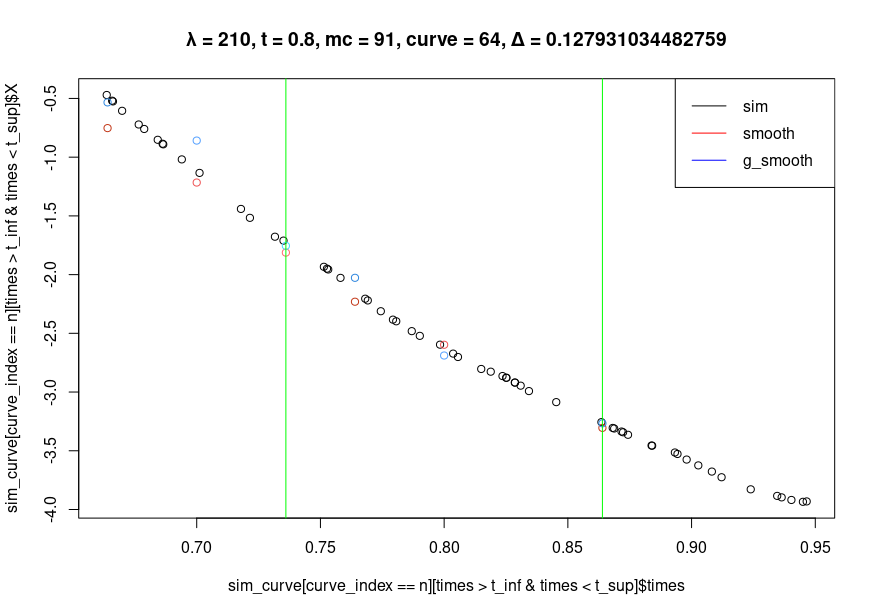
\includegraphics[width=0.47\textwidth]{Images/indiv_vs_glob/lbd210_mc91_c64.png}
	\end{minipage}
	\caption{Distribution des risques et aperçu d'une courbe pour un échantillon de monte carlo extrême sur le risque euclidien.}
	\label{fig:dist_R_eucl_curves}
\end{figure}

En regardant la densité de points présents sur l'intervalle $\mathcal T$, en utilisant un estimateur de Parzen-Rosenblatt de fenêtre $\Delta$ utilisé pour calculer $X(t_1)$ et $X(t_3)$ :

\begin{equation*}
	\widehat f_T = \frac 1 N \sum\limits_{i=1}^N \frac 1 {M_i} \sum\limits_{m=1}^{M_i} K\left( \frac{t - T_i[\, m \, ]}{\Delta} \right)
\end{equation*}



\begin{figure}[H]
	\centering
	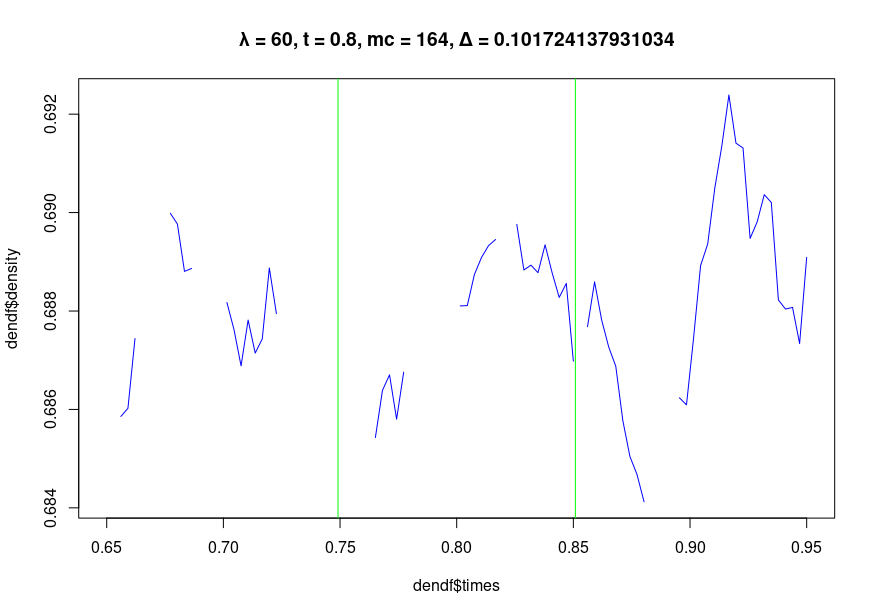
\includegraphics[width=0.7\textwidth]{Images/indiv_vs_glob/Tdensity_lbd60_mc164.png}
	\caption{Densité de points observés sur $[0.65, 0.95]$ pour $\lambda = 60$ sur un échantillon de monte carlo extrême, en un $\Delta$ problématique.}
	\label{fig:den_ex}
\end{figure}

Si cela semblerait être une cause plausible de la différence de comportement entre les deux méthodes, on pourrait fournir un contre-exemple à l'argument ssuivant. En effet en regardant cette fois la densité de points sur l'intervalle $\mathcal T$ pour un $\Delta=210$ lui aussi en un index de simulation de monte carlo extrême, on obtient la densité :

\begin{figure}[H]
	\centering
	\includegraphics[width=0.6\textwidth]{Images/indiv_vs_glob/}
	\caption{Densité des points observés correspondant à la courbe présentée sur la figure \ref{fig:dist_R_eucl_curves}.}
	\label{fig:den_counterex}
\end{figure}

De plus, là où il semblerait que